\begin{frame}[fragile]
    \begin{minted}[fontsize=\normalsize]{rust}
let results = b(Queens::new(4), 4);

pub fn b<T: Sequence>(initial: T, n: usize) -> Vec<T> {
    let mut results = Vec::new();
    let mut states = Vec::new();

    let steps = initial.next_steps().into_iter();
    states.push((initial, steps));
    // <- we are here
    // ...
}
    \end{minted}
    \ \\
    $results = [\ ]$ \\
    \ \\
    $states = [(\raisebox{-2ex}{
\includegraphics[height=\baselineskip * 2]{../img/empty.png}}, [
    
\includegraphics[height=\baselineskip / 2]{../img/step0.png},
    
\includegraphics[height=\baselineskip / 2]{../img/step1.png},
    
\includegraphics[height=\baselineskip / 2]{../img/step2.png},
    
\includegraphics[height=\baselineskip / 2]{../img/step3.png}])]$
\end{frame}
\begin{frame}[fragile]
    \begin{minted}{rust}
// ...
while let Some((state, steps)) = states.last_mut() {
    if let Some(step) = steps.next() {
        // <- we are here
        let next_state = state.apply_step(step);
        if next_state.satisfies_condition() {
            if states.len() < n {
                let next_steps = next_state.next_steps().into_iter();
                states.push((next_state, next_steps));
            } else {
                results.push(next_state);
            }
        }
    } else {
        states.pop();
    }
}
// ...
    \end{minted}
    $states = [(\raisebox{-2ex}{
\includegraphics[height=\baselineskip * 2]{../img/empty.png}}, [
    
\includegraphics[height=\baselineskip / 2]{../img/step1.png},
    
\includegraphics[height=\baselineskip / 2]{../img/step2.png},
    
\includegraphics[height=\baselineskip / 2]{../img/step3.png}])]$
    \ \\
    $step = 
\includegraphics[height=\baselineskip / 2]{../img/step0.png}$
\end{frame}
\begin{frame}[fragile]
    \begin{minted}{rust}
// ...
while let Some((state, steps)) = states.last_mut() {
    if let Some(step) = steps.next() {
        let next_state = state.apply_step(step);
        // <- we are here
        if next_state.satisfies_condition() {
            if states.len() < n {
                let next_steps = next_state.next_steps().into_iter();
                states.push((next_state, next_steps));
            } else {
                results.push(next_state);
            }
        }
    } else {
        states.pop();
    }
}
// ...
    \end{minted}
    $states = [(\raisebox{-2ex}{
\includegraphics[height=\baselineskip * 2]{../img/empty.png}}, [
    
\includegraphics[height=\baselineskip / 2]{../img/step1.png},
    
\includegraphics[height=\baselineskip / 2]{../img/step2.png},
    
\includegraphics[height=\baselineskip / 2]{../img/step3.png}])]$
    \ \\
    $next\_state = \raisebox{-2ex}{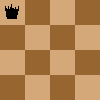
\includegraphics[height=\baselineskip * 2]{../img/state0.png}}$
\end{frame}
\begin{frame}[fragile]
    \begin{minted}{rust}
// ...
while let Some((state, steps)) = states.last_mut() {
    if let Some(step) = steps.next() {
        let next_state = state.apply_step(step);
        // our previous position
        if next_state.satisfies_condition() {
            if states.len() < n {
                let next_steps = next_state.next_steps().into_iter();
                states.push((next_state, next_steps));
                // <- we are here
            } else {
                results.push(next_state);
            }
        }
    } else {
        states.pop();
    }
}
// ...
    \end{minted}
    $states = [(\raisebox{-2ex}{
\includegraphics[height=\baselineskip * 2]{../img/empty.png}}, [
    
\includegraphics[height=\baselineskip / 2]{../img/step1.png},
    
\includegraphics[height=\baselineskip / 2]{../img/step2.png},
    
\includegraphics[height=\baselineskip / 2]{../img/step3.png}]),
    (\raisebox{-2ex}{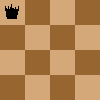
\includegraphics[height=\baselineskip * 2]{../img/state0.png}}, [
    
\includegraphics[height=\baselineskip / 2]{../img/step0.png},
    
\includegraphics[height=\baselineskip / 2]{../img/step1.png},
    
\includegraphics[height=\baselineskip / 2]{../img/step2.png},
    
\includegraphics[height=\baselineskip / 2]{../img/step3.png}])]$
\end{frame}
\begin{frame}[fragile]
    \begin{minted}{rust}
// ...
while let Some((state, steps)) = states.last_mut() {
    if let Some(step) = steps.next() {
        let next_state = state.apply_step(step);
        // <- we are here
        if next_state.satisfies_condition() {
            if states.len() < n {
                let next_steps = next_state.next_steps().into_iter();
                states.push((next_state, next_steps));
            } else {
                results.push(next_state);
            }
        }
    } else {
        states.pop();
    }
}
// ...
    \end{minted}
    $states = [(\raisebox{-2ex}{
\includegraphics[height=\baselineskip * 2]{../img/empty.png}}, [
    
\includegraphics[height=\baselineskip / 2]{../img/step1.png},
    
\includegraphics[height=\baselineskip / 2]{../img/step2.png},
    
\includegraphics[height=\baselineskip / 2]{../img/step3.png}]),
    (\raisebox{-2ex}{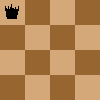
\includegraphics[height=\baselineskip * 2]{../img/state0.png}}, [
    
\includegraphics[height=\baselineskip / 2]{../img/step1.png},
    
\includegraphics[height=\baselineskip / 2]{../img/step2.png},
    
\includegraphics[height=\baselineskip / 2]{../img/step3.png}])]$ \ \\
    $next\_state = \raisebox{-2ex}{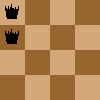
\includegraphics[height=\baselineskip * 2]{../img/state00.png}}$
\end{frame}
\begin{frame}[fragile]
    \begin{minted}{rust}
// ...
while let Some((state, steps)) = states.last_mut() {
    if let Some(step) = steps.next() {
        let next_state = state.apply_step(step);
        // <- we are here
        if next_state.satisfies_condition() {
            if states.len() < n {
                let next_steps = next_state.next_steps().into_iter();
                states.push((next_state, next_steps));
            } else {
                results.push(next_state);
            }
        }
    } else {
        states.pop();
    }
}
// ...
    \end{minted}
    $states = [(\raisebox{-2ex}{
\includegraphics[height=\baselineskip * 2]{../img/empty.png}}, [
    
\includegraphics[height=\baselineskip / 2]{../img/step1.png},
    
\includegraphics[height=\baselineskip / 2]{../img/step2.png},
    
\includegraphics[height=\baselineskip / 2]{../img/step3.png}]),
    (\raisebox{-2ex}{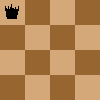
\includegraphics[height=\baselineskip * 2]{../img/state0.png}}, [
    
\includegraphics[height=\baselineskip / 2]{../img/step2.png},
    
\includegraphics[height=\baselineskip / 2]{../img/step3.png}])]$ \ \\
    $next\_state = \raisebox{-2ex}{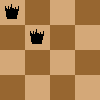
\includegraphics[height=\baselineskip * 2]{../img/state01.png}}$
\end{frame}
\begin{frame}[fragile]
    \begin{minted}{rust}
// ...
while let Some((state, steps)) = states.last_mut() {
    if let Some(step) = steps.next() {
        let next_state = state.apply_step(step);
        // <- we are here
        if next_state.satisfies_condition() {
            if states.len() < n {
                let next_steps = next_state.next_steps().into_iter();
                states.push((next_state, next_steps));
            } else {
                results.push(next_state);
            }
        }
    } else {
        states.pop();
    }
}
// ...
    \end{minted}
    $states = [(\raisebox{-2ex}{
\includegraphics[height=\baselineskip * 2]{../img/empty.png}}, [
    
\includegraphics[height=\baselineskip / 2]{../img/step1.png},
    
\includegraphics[height=\baselineskip / 2]{../img/step2.png},
    
\includegraphics[height=\baselineskip / 2]{../img/step3.png}]),
    (\raisebox{-2ex}{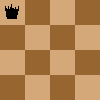
\includegraphics[height=\baselineskip * 2]{../img/state0.png}}, [
    
\includegraphics[height=\baselineskip / 2]{../img/step3.png}])]$ \ \\
    $next\_state = \raisebox{-2ex}{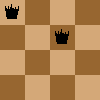
\includegraphics[height=\baselineskip * 2]{../img/state02.png}}$
\end{frame}
\begin{frame}[fragile]
    \begin{minted}{rust}
while let Some((state, steps)) = states.last_mut() {
    if let Some(step) = steps.next() {
        let next_state = state.apply_step(step);
        if next_state.satisfies_condition() {
            if states.len() < n {
                let next_steps = next_state.next_steps().into_iter();
                states.push((next_state, next_steps));
                // <- we are here
            } else {
                results.push(next_state);
            }
        }
    } else {
        states.pop();
    }
}
    \end{minted}
    $states = [(\raisebox{-2ex}{
\includegraphics[height=\baselineskip * 2]{../img/empty.png}}, [
    
\includegraphics[height=\baselineskip / 2]{../img/step1.png},
    \includegraphics[height=\baselineskip / 2]{../img/step2.png},
    \includegraphics[height=\baselineskip / 2]{../img/step3.png}]
    ),
    (\raisebox{-2ex}{\includegraphics[height=\baselineskip * 2]{../img/state0.png}}, [
    \includegraphics[height=\baselineskip / 2]{../img/step3.png}]
    ), \\
    (\raisebox{-2ex}{\includegraphics[height=\baselineskip * 2]{../img/state02.png}}, [
    \includegraphics[height=\baselineskip / 2]{../img/step0.png},
    \includegraphics[height=\baselineskip / 2]{../img/step1.png},
    \includegraphics[height=\baselineskip / 2]{../img/step2.png},
    \includegraphics[height=\baselineskip / 2]{../img/step3.png}]
    )]$ \ \\
\end{frame}
\begin{frame}[fragile]
    \begin{minted}{rust}
while let Some((state, steps)) = states.last_mut() {
    // <- we are here after discarding all 4 steps
    if let Some(step) = steps.next() {
        let next_state = state.apply_step(step);
        if next_state.satisfies_condition() {
            if states.len() < n {
                let next_steps = next_state.next_steps().into_iter();
                states.push((next_state, next_steps));
            } else {
                results.push(next_state);
            }
        }
    } else {
        states.pop();
    }
}
    \end{minted}
    $states = [(\raisebox{-2ex}{\includegraphics[height=\baselineskip * 2]{../img/empty.png}}, [
    \includegraphics[height=\baselineskip / 2]{../img/step1.png},
    \includegraphics[height=\baselineskip / 2]{../img/step2.png},
    \includegraphics[height=\baselineskip / 2]{../img/step3.png}]
    ),
    (\raisebox{-2ex}{\includegraphics[height=\baselineskip * 2]{../img/state0.png}}, [
    \includegraphics[height=\baselineskip / 2]{../img/step3.png}]
    ),
    (\raisebox{-2ex}{\includegraphics[height=\baselineskip * 2]{../img/state02.png}}, [\ ])]$ \ \\
\end{frame}
\begin{frame}[fragile]
    \begin{minted}{rust}
while let Some((state, steps)) = states.last_mut() {
    if let Some(step) = steps.next() {
        let next_state = state.apply_step(step);  
        if next_state.satisfies_condition() {
            if states.len() < n {
                let next_steps = next_state.next_steps().into_iter();
                states.push((next_state, next_steps));
            } else {
                results.push(next_state);
            }
        }
    } else {
        states.pop();
        // <- we are here
    }
}
    \end{minted}
    $states = [(\raisebox{-2ex}{\includegraphics[height=\baselineskip * 2]{../img/empty.png}}, [
    \includegraphics[height=\baselineskip / 2]{../img/step1.png},
    \includegraphics[height=\baselineskip / 2]{../img/step2.png},
    \includegraphics[height=\baselineskip / 2]{../img/step3.png}]
    ),
    (\raisebox{-2ex}{\includegraphics[height=\baselineskip * 2]{../img/state0.png}}, [
    \includegraphics[height=\baselineskip / 2]{../img/step3.png}]
    )]$ \ \\
\end{frame}
\begin{frame}[fragile]
    \begin{minted}{rust}
while let Some((state, steps)) = states.last_mut() {
    if let Some(step) = steps.next() {
        let next_state = state.apply_step(step);
        // <- we are here
        if next_state.satisfies_condition() {
            if states.len() < n {
                let next_steps = next_state.next_steps().into_iter();
                states.push((next_state, next_steps));
            } else {
                results.push(next_state);
            }
        }
    } else {
        states.pop();
    }
}
    \end{minted}
    $states = [(\raisebox{-2ex}{\includegraphics[height=\baselineskip * 2]{../img/empty.png}}, [
    \includegraphics[height=\baselineskip / 2]{../img/step1.png},
    \includegraphics[height=\baselineskip / 2]{../img/step2.png},
    \includegraphics[height=\baselineskip / 2]{../img/step3.png}]
    ),
    (\raisebox{-2ex}{\includegraphics[height=\baselineskip * 2]{../img/state0.png}}, [\ ])]$ \ \\
    $next\_state = \raisebox{-2ex}{\includegraphics[height=\baselineskip * 2]{../img/state03.png}}$
\end{frame}
\begin{frame}[fragile]
    \begin{minted}{rust}
while let Some((state, steps)) = states.last_mut() {
    if let Some(step) = steps.next() {
        let next_state = state.apply_step(step);
        // <- we are here
        if next_state.satisfies_condition() {
            if states.len() < n {
                let next_steps = next_state.next_steps().into_iter();
                states.push((next_state, next_steps));
            } else {
                results.push(next_state);
            }
        }
    } else {
        states.pop();
    }
}
    \end{minted}
    $states = [(\raisebox{-2ex}{\includegraphics[height=\baselineskip * 2]{../img/empty.png}}, [
    \includegraphics[height=\baselineskip / 2]{../img/step1.png},
    \includegraphics[height=\baselineskip / 2]{../img/step2.png},
    \includegraphics[height=\baselineskip / 2]{../img/step3.png}]
    ),
    (\raisebox{-2ex}{\includegraphics[height=\baselineskip * 2]{../img/state0.png}}, [\ ]),
    (\raisebox{-2ex}{\includegraphics[height=\baselineskip * 2]{../img/state03.png}}, [
    \includegraphics[height=\baselineskip / 2]{../img/step2.png},
    \includegraphics[height=\baselineskip / 2]{../img/step3.png}])]$ \ \\
    $next\_state = \raisebox{-2ex}{\includegraphics[height=\baselineskip * 2]{../img/state031.png}}$
\end{frame}
\begin{frame}[fragile]
    \begin{minted}{rust}
while let Some((state, steps)) = states.last_mut() {
    if let Some(step) = steps.next() {
        let next_state = state.apply_step(step);
        if next_state.satisfies_condition() {
            if states.len() < n {
                let next_steps = next_state.next_steps().into_iter();
                states.push((next_state, next_steps));
            } else {
                results.push(next_state);
            }
        }
    } else { 
        states.pop();
        // <- we are here
    }
}
    \end{minted}
    $states = [(\raisebox{-2ex}{\includegraphics[height=\baselineskip * 2]{../img/empty.png}}, [
    \includegraphics[height=\baselineskip / 2]{../img/step1.png},
    \includegraphics[height=\baselineskip / 2]{../img/step2.png},
    \includegraphics[height=\baselineskip / 2]{../img/step3.png}]
    ),
    (\raisebox{-2ex}{\includegraphics[height=\baselineskip * 2]{../img/state0.png}}, [\ ]),
    (\raisebox{-2ex}{\includegraphics[height=\baselineskip * 2]{../img/state03.png}}, [
    \includegraphics[height=\baselineskip / 2]{../img/step2.png},
    \includegraphics[height=\baselineskip / 2]{../img/step3.png}])]$ \ \\
\end{frame}
\begin{frame}[fragile]
    \begin{minted}{rust}
while let Some((state, steps)) = states.last_mut() {
    if let Some(step) = steps.next() {
        let next_state = state.apply_step(step);
        if next_state.satisfies_condition() {
            if states.len() < n {
                let next_steps = next_state.next_steps().into_iter();
                states.push((next_state, next_steps));
            } else {
                results.push(next_state);
            }
        }
    } else { 
        states.pop();
        // <- we are here
    }
}
    \end{minted}
    $states = [(\raisebox{-2ex}{\includegraphics[height=\baselineskip * 2]{../img/empty.png}}, [
    \includegraphics[height=\baselineskip / 2]{../img/step1.png},
    \includegraphics[height=\baselineskip / 2]{../img/step2.png},
    \includegraphics[height=\baselineskip / 2]{../img/step3.png}]
    ),
    (\raisebox{-2ex}{\includegraphics[height=\baselineskip * 2]{../img/state0.png}}, [\ ]),]$ \ \\
\end{frame}
\begin{frame}[fragile]
    \begin{minted}{rust}
while let Some((state, steps)) = states.last_mut() {
    if let Some(step) = steps.next() {
        let next_state = state.apply_step(step);
        if next_state.satisfies_condition() {
            if states.len() < n {
                let next_steps = next_state.next_steps().into_iter();
                states.push((next_state, next_steps));
                // <- we are here
            } else {
                results.push(next_state);
            }
        }
    } else { 
        states.pop();
    }
}
    \end{minted}
    $states = [(\raisebox{-2ex}{\includegraphics[height=\baselineskip * 2]{../img/empty.png}}, [
    \includegraphics[height=\baselineskip / 2]{../img/step2.png},
    \includegraphics[height=\baselineskip / 2]{../img/step3.png}]
    ),
    (\raisebox{-2ex}{\includegraphics[height=\baselineskip * 2]{../img/state1.png}}, [
    \includegraphics[height=\baselineskip / 2]{../img/step0.png},
    \includegraphics[height=\baselineskip / 2]{../img/step1.png},
    \includegraphics[height=\baselineskip / 2]{../img/step2.png},
    \includegraphics[height=\baselineskip / 2]{../img/step3.png}])]$ \ \\
\end{frame}
\begin{frame}[fragile]
    \begin{minted}{rust}
while let Some((state, steps)) = states.last_mut() {
    if let Some(step) = steps.next() {
        let next_state = state.apply_step(step);
        if next_state.satisfies_condition() {
            // <- we are here
            if states.len() < n {
                let next_steps = next_state.next_steps().into_iter();
                states.push((next_state, next_steps));
            } else {
                results.push(next_state);
            }
        }
    } else { 
        states.pop();
    }
}
    \end{minted}
    $states = [(\raisebox{-2ex}{\includegraphics[height=\baselineskip * 2]{../img/empty.png}}, [
    \includegraphics[height=\baselineskip / 2]{../img/step2.png},
    \includegraphics[height=\baselineskip / 2]{../img/step3.png}]
    ),
    (\raisebox{-2ex}{\includegraphics[height=\baselineskip * 2]{../img/state1.png}}, [\ ]),
    (\raisebox{-2ex}{\includegraphics[height=\baselineskip * 2]{../img/state13.png}}, [
    \includegraphics[height=\baselineskip / 2]{../img/step1.png},
    \includegraphics[height=\baselineskip / 2]{../img/step2.png},
    \includegraphics[height=\baselineskip / 2]{../img/step3.png}]
    ), \\
    (\raisebox{-2ex}{\includegraphics[height=\baselineskip * 2]{../img/state130.png}}, [
    \includegraphics[height=\baselineskip / 2]{../img/step3.png}]
    )]$ \ \\
    $next\_state = \raisebox{-2ex}{\includegraphics[height=\baselineskip * 2]{../img/state1302.png}}$
\end{frame}
\begin{frame}[fragile]
    \begin{minted}{rust}
while let Some((state, steps)) = states.last_mut() {
    if let Some(step) = steps.next() {
        let next_state = state.apply_step(step);
        if next_state.satisfies_condition() {
            if states.len() < n {
                let next_steps = next_state.next_steps().into_iter();
                states.push((next_state, next_steps));
            } else {
                results.push(next_state);
                // <- we are here
            }
        }
    } else { 
        states.pop();
    }
}
    \end{minted}
    $states = [(\raisebox{-2ex}{\includegraphics[height=\baselineskip * 2]{../img/empty.png}}, [
    \includegraphics[height=\baselineskip / 2]{../img/step2.png},
    \includegraphics[height=\baselineskip / 2]{../img/step3.png}]
    ),
    (\raisebox{-2ex}{\includegraphics[height=\baselineskip * 2]{../img/state1.png}}, [\ ]),
    (\raisebox{-2ex}{\includegraphics[height=\baselineskip * 2]{../img/state13.png}}, [
    \includegraphics[height=\baselineskip / 2]{../img/step1.png},
    \includegraphics[height=\baselineskip / 2]{../img/step2.png},
    \includegraphics[height=\baselineskip / 2]{../img/step3.png}]
    ), \\
    (\raisebox{-2ex}{\includegraphics[height=\baselineskip * 2]{../img/state130.png}}, [
    \includegraphics[height=\baselineskip / 2]{../img/step3.png}]
    )]$ \ \\
    $results = [\raisebox{-2ex}{\includegraphics[height=\baselineskip * 2]{../img/state1302.png}}]$
\end{frame}
\begin{frame}[fragile]
    \begin{minted}{rust}
while let Some((state, steps)) = states.last_mut() {
    if let Some(step) = steps.next() {
        let next_state = state.apply_step(step);
        if next_state.satisfies_condition() {
            if states.len() < n {
                let next_steps = next_state.next_steps().into_iter();
                states.push((next_state, next_steps));
            } else {
                results.push(next_state);
                // <- we are here
            }
        }
    } else { 
        states.pop();
    }
}
    \end{minted}
    $states = [(\raisebox{-2ex}{\includegraphics[height=\baselineskip * 2]{../img/empty.png}}, [
    \includegraphics[height=\baselineskip / 2]{../img/step3.png}]
    ),
    (\raisebox{-2ex}{\includegraphics[height=\baselineskip * 2]{../img/state2.png}}, [
    \includegraphics[height=\baselineskip / 2]{../img/step1.png},
    \includegraphics[height=\baselineskip / 2]{../img/step2.png},
    \includegraphics[height=\baselineskip / 2]{../img/step3.png}
    ]),
    (\raisebox{-2ex}{\includegraphics[height=\baselineskip * 2]{../img/state20.png}}, [\ ]), \\
    (\raisebox{-2ex}{\includegraphics[height=\baselineskip * 2]{../img/state203.png}}, [
    \includegraphics[height=\baselineskip / 2]{../img/step2.png},
    \includegraphics[height=\baselineskip / 2]{../img/step3.png}]
    )]$ \ \\
    $results = [
    \raisebox{-2ex}{\includegraphics[height=\baselineskip * 2]{../img/state1302.png}},
    \raisebox{-2ex}{\includegraphics[height=\baselineskip * 2]{../img/state2031.png}}
    ]$
\end{frame}
\begin{frame}[fragile]
    \begin{minted}{rust}
while let Some((state, steps)) = states.last_mut() {
    if let Some(step) = steps.next() {
        let next_state = state.apply_step(step);
        if next_state.satisfies_condition() {
            if states.len() < n {
                let next_steps = next_state.next_steps().into_iter();
                states.push((next_state, next_steps));
            } else {
                results.push(next_state);      
            }
        }
    } else { 
        states.pop();
        // <- we are here
    }
}
    \end{minted}
    $states = [(\raisebox{-2ex}{\includegraphics[height=\baselineskip * 2]{../img/empty.png}}, [\ ])]$
\end{frame}
\begin{frame}[fragile]
    \begin{minted}{rust}
while let Some((state, steps)) = states.last_mut() {
    if let Some(step) = steps.next() {
        let next_state = state.apply_step(step);
        if next_state.satisfies_condition() {
            if states.len() < n {
                let next_steps = next_state.next_steps().into_iter();
                states.push((next_state, next_steps));
            } else {
                results.push(next_state);      
            }
        }
    } else { 
        states.pop();
        // <- we are here
    }
}
    \end{minted}
    $states = [\ ]$
\end{frame}
\begin{frame}[fragile]
    \begin{minted}{rust}
while let Some((state, steps)) = states.last_mut() {
    if let Some(step) = steps.next() {
        let next_state = state.apply_step(step);
        if next_state.satisfies_condition() {
            if states.len() < n {
                let next_steps = next_state.next_steps().into_iter();
                states.push((next_state, next_steps));
            } else {
                results.push(next_state);      
            }
        }
    } else { 
        states.pop();
    }
}
// <- we are here
results
    \end{minted}
    $states = [\ ]$ \\
    \ \\
    $results = [
    \raisebox{-2ex}{\includegraphics[height=\baselineskip * 2]{../img/state1302.png}},
    \raisebox{-2ex}{\includegraphics[height=\baselineskip * 2]{../img/state2031.png}}
    ]$
\end{frame}